% Created 2023-03-01 Wed 19:22
% Intended LaTeX compiler: pdflatex
\documentclass[11pt]{article}
\usepackage[utf8]{inputenc}
\usepackage[T1]{fontenc}
\usepackage{graphicx}
\usepackage{longtable}
\usepackage{wrapfig}
\usepackage{rotating}
\usepackage[normalem]{ulem}
\usepackage{amsmath}
\usepackage{amssymb}
\usepackage{capt-of}
\usepackage{hyperref}
\author{Diego Domínguez}
\date{\today}
\title{}
\hypersetup{
 pdfauthor={Diego Domínguez},
 pdftitle={},
 pdfkeywords={},
 pdfsubject={},
 pdfcreator={Emacs 28.2 (Org mode 9.6)}, 
 pdflang={English}}
\begin{document}

\tableofcontents

\#*OPTIONS: toc:nil
\#*LATEX\textsubscript{HEADER}: \begin{center}
	\includegraphics[scale=0.25]{/home/dieguito/Pictures/logo_udeg_negro.png}\\
	\vspace{1cm}
{\Large 	\textbf{Centro Universitario de Ciencias Exactas e Ingenierías}\\}

\vspace{0.5cm}
	
{\large 	\textit{Departamento de ciencias computacionales}\\}
	
	\vspace{1cm}
	
	\textbf{Administración de redes}\\
	
	\vspace{0.5cm}
	
	\textbf{Reporte semanal}\\
	
	\vspace{0.5cm}
	
	Semana \textbf{7}
	
	\vspace{0.5cm}
	
	\underline{Packet tracer}\\
	
	\vspace{1cm}
	
	Prof: Ing. Luis Ignacio Sánchez Salazar\\
	
	Alumno: Diego Martín Domínguez Hernández\\
	
	Carrera: Ingeniería Informática \\
	
	Materia: i5907 (Administración de Redes)\\
	
	NRC: 42241\\
	
	Sección: D04\\

	Calendario: 2023A\\
	
\end{center}
\newpage


\begin{itemize}
\item Establecer
\begin{itemize}
\item Máscaras
\item Red
\item Broadcast
\item Rango útil
\item Red
\end{itemize}
\end{itemize}

\begin{center}
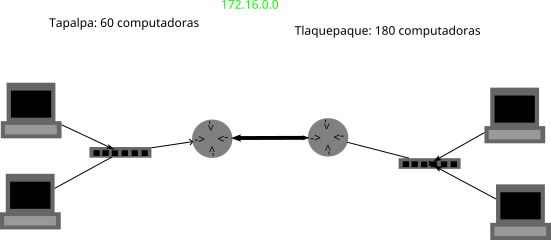
\includegraphics[width=.9\linewidth]{./ejercicio.png}
\end{center}


\section{Tlaquepaque}
\label{sec:orgaf0c3e6}
\begin{itemize}
\item Network: 172.16.0.0
\item Mask: 255.255.255.0
\item Broadcast: 172.16.0.255
\item Rango útil: 172.16.0.1 -> 172.16.0.254
\item Gateway: 172.16.0.254
\end{itemize}

\section{Tapalpa}
\label{sec:orgc82810c}
\begin{itemize}
\item Network: 172.16.1.0
\item Mask: 255.255.255.192
\item Broadcast: 172.16.1.63
\item Rango útil: 172.16.1.1 -> 172.16.1.62
\item Gateway: 172.16.1.62
\end{itemize}

\section{Enlace Tapalpa - Tlaquepaque}
\label{sec:org6e79ca9}
\begin{itemize}
\item Network: 172.16.1.64
\item Mask: 255.255.255.252
\item Broadcast: 172.16.1.67
\item Rango útil: 172.16.1.65 -> 172.16.1.66
\end{itemize}

\begin{center}
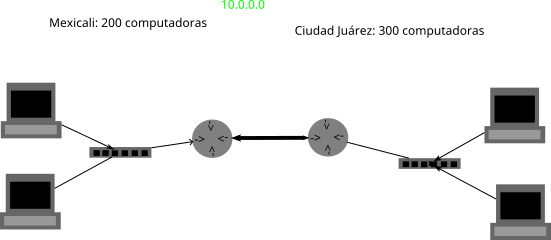
\includegraphics[width=.9\linewidth]{./ejercicio2.png}
\end{center}

\section{Ciudad Juárez}
\label{sec:org52775ec}
\begin{itemize}
\item Network: 10.0.0.0
\item Mask: 255.255.254.0
\item Broadcast: 10.0.1.255
\item Rango útil: 10.0.1.254 -> 10.0.1.254
\item Gateway: 10.0.1.254
\end{itemize}

\section{Mexicali}
\label{sec:org1c023ac}
\begin{itemize}
\item Network: 10.0.3.0
\item Mask: 255.255.255.252
\item Broadcast: 10.0.3.3
\item Rango útil: 10.0.3.1 -> 10.0.3.2
\item Gateway: 10.0.4.254
\end{itemize}


También se vio cómo utilizar \emph{IP Network
Calculator}, una aplicación de la Play Store que
estima las variables que utilizamos en clase, es
muy intuitiva y muchísimo más fácil de utilizar
que realizar los cálculos uno a uno.

\begin{center}
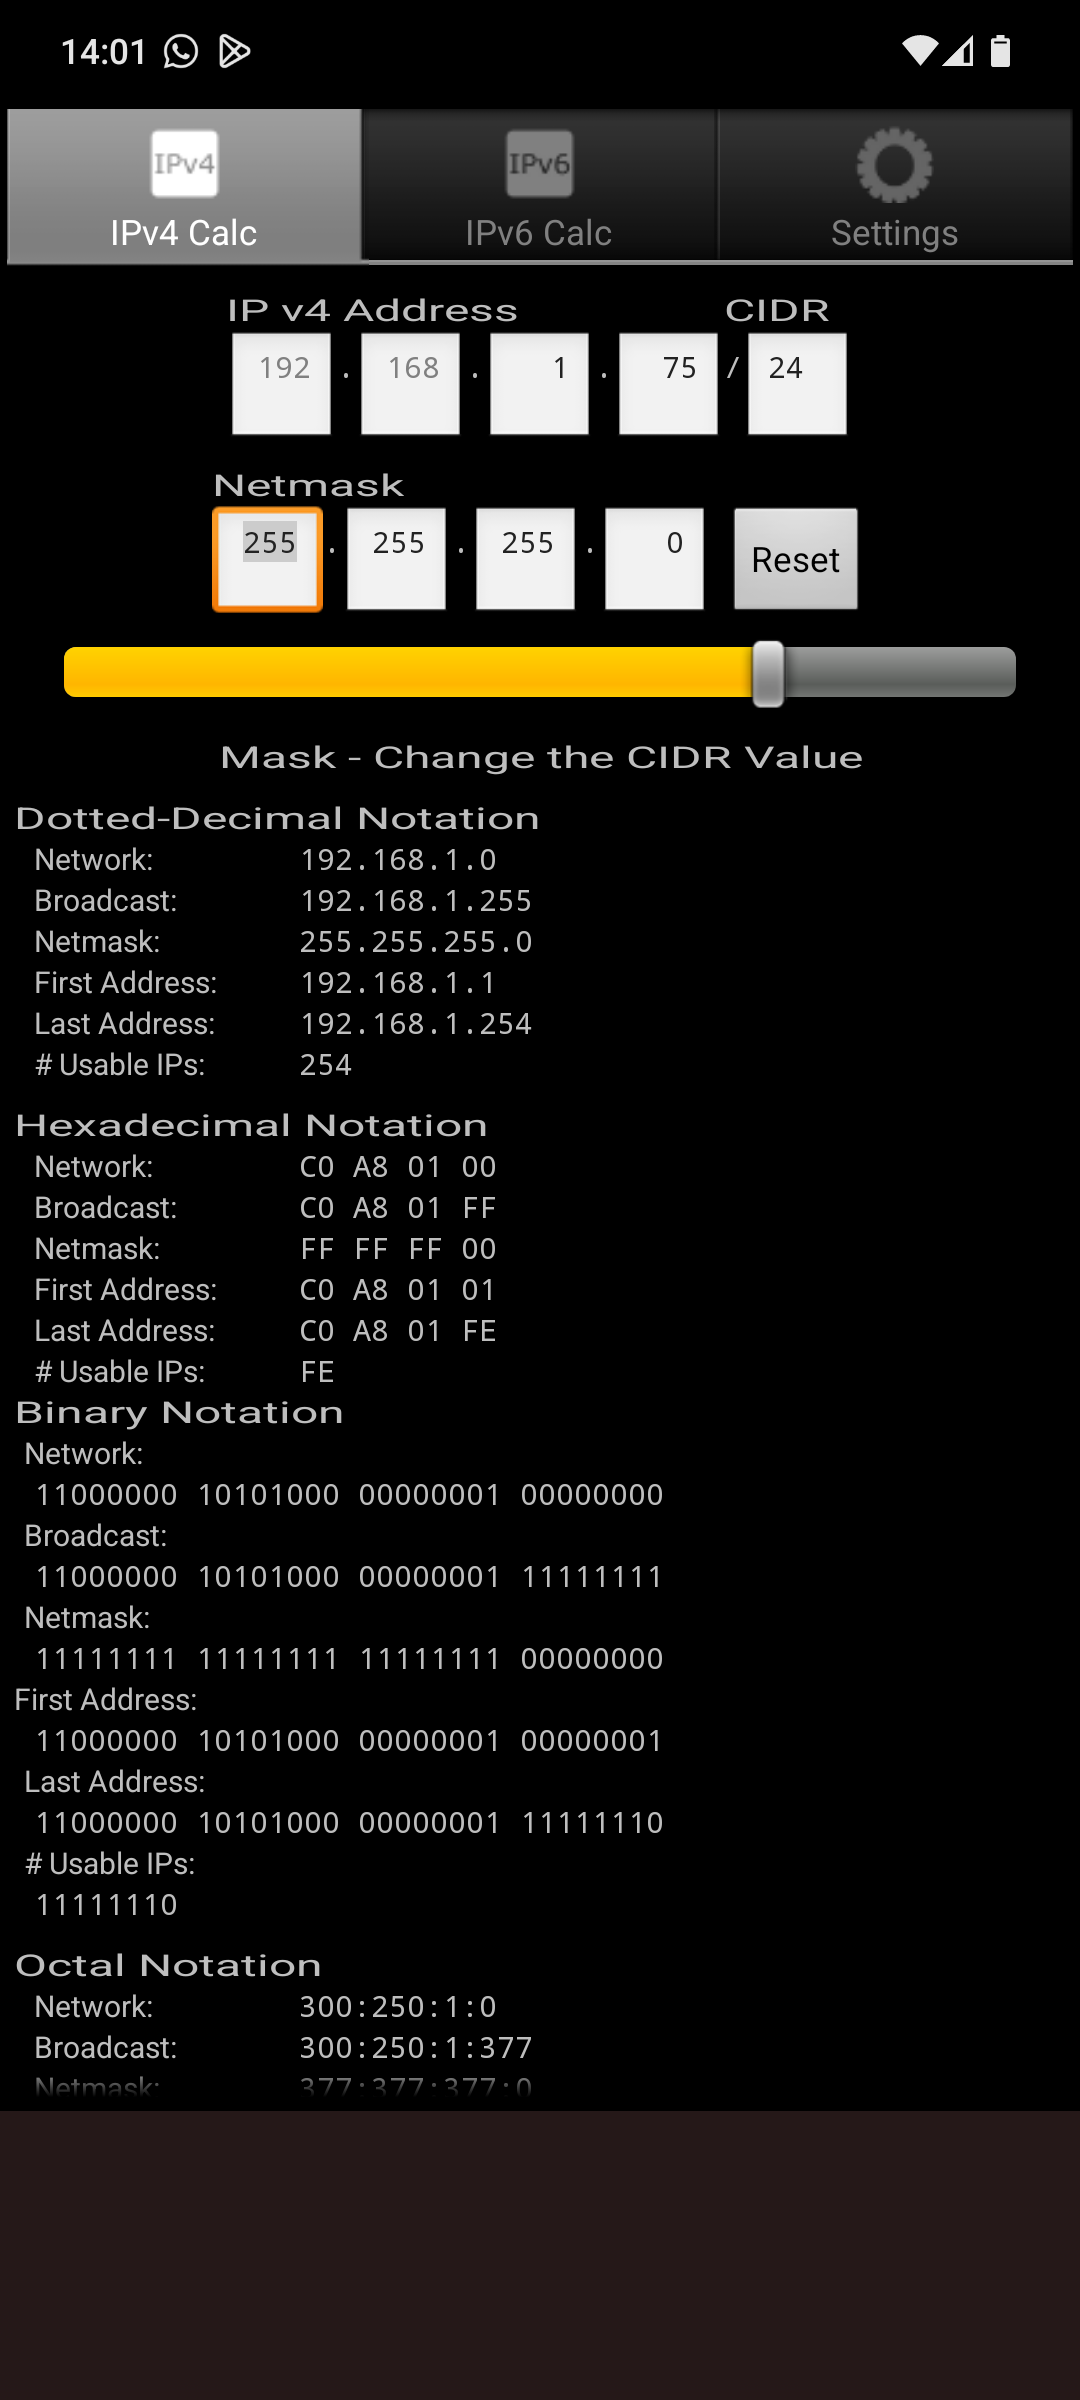
\includegraphics[width=200px]{./IpvCalc.png}
\end{center}
\end{document}